\let\clearforchapter\par % cheating, but saves some space


\chapter{Data Types}
\label{ch:datatypes}


Those familiar with programming in C should find Scout's syntax and fundamental data 
types to be very familiar.  In this section we quickly review Scout's additional composite data types.

\section{Vectors}
\label{ch:vectors}

As briefly mentioned in Section~\ref{ch1:scout-clang}, Scout provides support for two-, three-, 
and four-component vector types.  The "base" type for vectors includes signed and unsigned 
values of each of the fundamental types (\texttt{bool}, \texttt{char}, \texttt{short}, 
\texttt{int}, \texttt{long}, \texttt{float}, \texttt{double}).  The syntax for defining a 
vector uses these types followed by the number of components in the vector. Listing~\ref{lst-vector} 
shows some example vector declarations and initializations.

\par\bigskip
\begin{lstlisting}[float=h,label=lst-vector,
    caption={Vector declarations and initialization.}]
// Vector declarations
float2  u; // two-component single-precision vector.
int3    v; // three-component integer vector.
double4 w; // four-component double-precision vector.

// Vector declaration and initialization
float3 foo = (float3){1.0f, 2.0f, 3.0f};

// Another way to initialize a vector
float4 bar;
bar.x = 1.0f;
bar.y = 2.0f;
bar.z = 3.0f;
bar.w = 4.0f;
\end{lstlisting}
\par\bigskip\noindent

\section{Meshes}
\label{ch:meshes}

Computational science data structures are frequently based on the concept of a mesh.
Scout directly follows this philosophy by introducing mesh-centric data types.  Scout supports 
the \texttt{uniform} mesh type.  

%\texttt{rectilinear}, \texttt{structured}, and \texttt{unstructured} 

In addition, the language 
provides constructs for defining the values stored on the various locations of the mesh (e.g.
cell centers, vertices, edges and faces).  Figure~\ref{fig:types:mesh-def} illustrates the layout of a mesh.
Figure~\ref{fig:types:grid-positions} shows the field placement options within a mesh.

\par\bigskip
\begin{figure}[h]
  \centering
  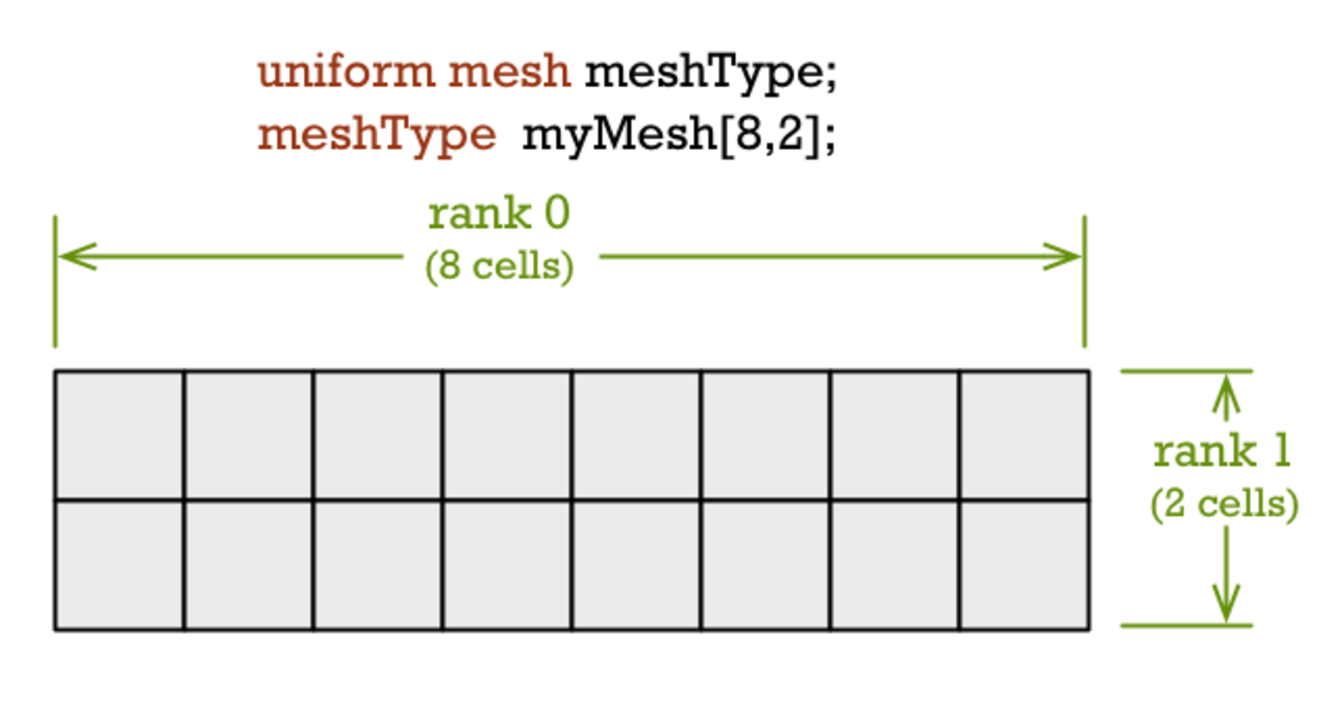
\includegraphics[width=4.0in]{datatypes/figures/mesh-def.pdf} \\
  \caption{Example of a uniform mesh definition.}
  \label{fig:types:mesh-def}
\end{figure}



\begin{figure}[h]
  \centering
  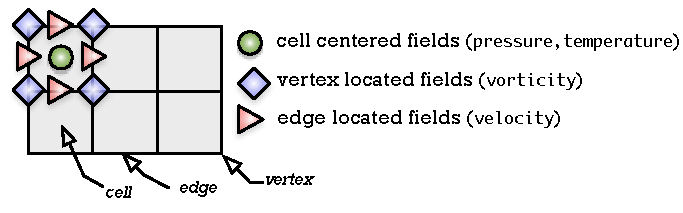
\includegraphics[width=4.0in]{datatypes/figures/field-positions.pdf} \\
  \caption{Field placement options within a mesh.}
  \label{fig:types:grid-positions}
\end{figure}
\par\bigskip\noindent

%TODO:  need a 2D picture that shows faces.

Here is a code example showing a two-dimensional mesh and a mesh
whose dimensions are defined by an input file.
Listing~\ref{lst-mesh} shows some example mesh declarations.
Note that is is not yet implemented to read meshes from input files.

\par\bigskip
\begin{lstlisting}[float=h,label=lst-mesh,
    caption={Mesh declarations.}]
// Two-dimensional uniform mesh with values stored at cell 
// centers and cell verticies. 
uniform mesh MeshType {
	cells:    float temperature;
	          float presure;
	vertices: float3 vorticity;
  edges:    float  velocity;
};

MeshType myMesh[512,512];

\end{lstlisting}
\par\bigskip\noindent


In addition, meshes dimensions can be specified using variables.
Listing~\ref{lst-meshvar} shows this.

\par\bigskip
\begin{lstlisting}[float=h,label=lst-meshvar,
    caption={Mesh declarations using variable.}]
  int dim = 4;

  uniform mesh HeatMeshType{
  cells:
    float t1, t2;
  };

  HeatMeshType heat_mesh[dim];
\end{lstlisting}
\par\bigskip\noindent


%Note: need examples here of how to declare rectilinear, structured and unstructured meshes.
